\appendix
\newpage
\section{Appendix}

\subsection{Verdict Tags in AITA and AITAH}
\label{sec:appendix-tags}

Both communities ask commenters to open a top-level reply with one of seven
verdict tags (Table~\ref{tab:tags}). Six of them assign blame and enter the
analysis; \emph{INFO} alone declines to judge and is discarded. \emph{YWBTA}
and \emph{YWNBTA} are the hypothetical forms, used when the OP asks about an
action not yet taken rather than one already taken; because they point the
blame in the same direction as \emph{NTA} and \emph{YTA}, they join those tags
in the exculpating group $\mathrm{NA}$ and the inculpating group $\mathrm{YA}$
respectively (\S\ref{subsec:dataset}).

The vocabularies are otherwise identical, with one difference in surface form:
AITAH additionally accepts H-suffixed aliases of the four OP-directed tags
(\emph{NTAH}, \emph{YTAH}, \emph{YWNBTAH}, \emph{YWBTAH}), which we normalise to
their unsuffixed counterparts before any analysis. \emph{NAH}, \emph{ESH}, and
\emph{INFO} have no suffixed variant in either community.

\begin{table}[th]
  \centering
  \small
  \begin{tabular}{@{}llp{0.6\columnwidth}@{}}
    \toprule
    Tag & Group & Meaning \\
    \midrule
    NTA     & $\mathrm{NA}$ & Not the Asshole---the OP is not, and the other person is \\
    YWNBTA  & $\mathrm{NA}$ & You Would Not Be the Asshole---as \emph{NTA}, for an action not yet taken \\
    NAH     & $\mathrm{NA}$ & No Assholes Here---nobody in the situation is at fault \\
    \addlinespace[2pt]
    YTA     & $\mathrm{YA}$ & You're the Asshole---the OP is, and the other person is not \\
    YWBTA   & $\mathrm{YA}$ & You Would Be the Asshole---as \emph{YTA}, for an action not yet taken \\
    ESH     & $\mathrm{YA}$ & Everyone Sucks Here---the OP and the other parties are all at fault \\
    \addlinespace[2pt]
    INFO    & ---           & Not Enough Info---more detail is needed to judge \\
    \bottomrule
  \end{tabular}
  \caption{The verdict tags shared by AITA and AITAH. Six assign blame and are
  grouped into the exculpating group
  $\mathrm{NA}=\{\text{NTA},\text{YWNBTA},\text{NAH}\}$ and the inculpating
  group $\mathrm{YA}=\{\text{YTA},\text{YWBTA},\text{ESH}\}$; \emph{INFO}
  states no judgment and is discarded. AITAH also accepts H-suffixed
  aliases of the four OP-directed tags (\emph{NTAH}, \emph{YTAH},
  \emph{YWNBTAH}, \emph{YWBTAH}), normalised to the forms shown here.}
  \label{tab:tags}
\end{table}


\subsection{Post-Content Comparability}
\label{sec:appendix-content}

The two communities discuss substantially, but not identically, the same
situations. A classifier recovering a post's source community from its
embedding alone reaches a ROC-AUC of $0.613$ under BGE and $0.568$ under E5,
against a chance level of $0.50$, and the UMAP projection in
Figure~\ref{fig:umap} shows why: the two communities interleave throughout the
map, including within the small peripheral clusters that correspond to
recurring situation types.

The difference that remains is nonetheless systematic rather than noise.
Maximum mean discrepancy and energy-distance tests reject equality of the two
embedding distributions under both encoders (permutation $p=.005$ in every
case). Topic modelling locates the difference in composition rather than in
kind: the communities share most topics, but AITAH leans towards romantic and
intimate relationships, while AITA carries relatively more everyday disputes
over housing, money, food, transport, and family obligation (Jensen--Shannon
distance between the topic distributions $0.187$ under BGE, $0.206$ under E5).

We therefore do not treat the two communities as topically interchangeable, and
the design does not require it. The paired analysis of
\S\ref{subsec:res-duplicates} holds the story itself fixed, comparing how two
crowds judge the same text, and for the unpaired analyses we treat
\emph{agreement} across the communities, rather than their raw difference, as
the evidential unit (\S\ref{subsec:method}).

\begin{figure}[t]
  \centering
  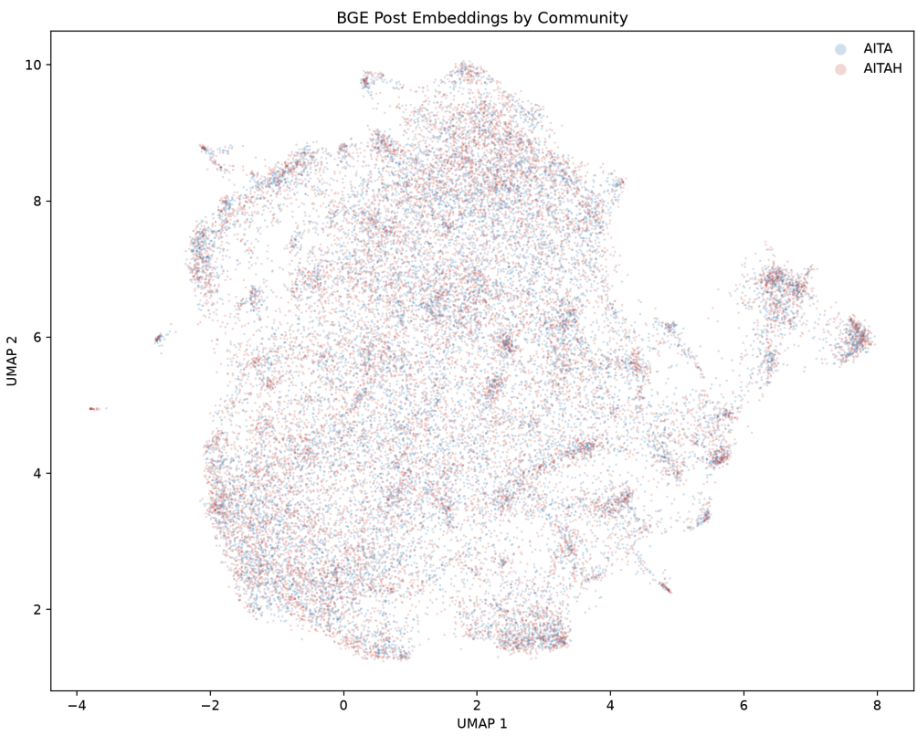
\includegraphics[width=\columnwidth]{figures/embeddings.png}
  \caption{Topical overlap between AITA and AITAH. $768$-dimensional
  \texttt{bge-base-en-v1.5} embeddings of post texts, projected to two
  dimensions with UMAP and colored by source community. The two communities
  interleave rather than separate, including within the small peripheral
  clusters, and community is only weakly recoverable from these embeddings
  (ROC-AUC $0.613$; $0.568$ under E5, chance $=0.50$)---though distributional
  tests still detect a reliable difference in topic composition.}
  \label{fig:umap}
\end{figure}


\subsection{Cross-Community User Overlap}
\label{sec:appendix-overlap}

Table~\ref{tab:shared-users} reports the user overlap between AITA and AITAH
within the aligned window of \S\ref{subsec:dataset}, under several definitions
of what counts as a member of a community. The pattern discussed in the main
text is stable across all of them: roughly a fifth of the combined user base is
active in both communities, and tightening the cohort to heavier or
longer-tenured users does not change that, whereas the overlap among story
authors is an order of magnitude smaller.



\begin{table}[t]
  \centering
  \begin{tabular}{@{}lrr@{}}
    \toprule
    User cohort & Shared users & Jaccard \\
    \midrule
    All users                    & $1{,}081{,}782$ & $20.3\%$ \\
    Users who posted             & $39{,}010$      & $4.3\%$  \\
    At least 10 activities       & $194{,}843$     & $18.5\%$ \\
    At least 100 activities      & $23{,}893$      & $16.2\%$ \\
    Active for at least 30 days  & $459{,}720$     & $23.6\%$ \\
    Active for at least one year & $183{,}825$     & $21.3\%$ \\
    \bottomrule
  \end{tabular}
  \caption{Users shared between AITA and AITAH within the aligned window, by
  cohort. Jaccard overlap is the shared count divided by the union of the two
  communities' user sets for that cohort. \emph{Activities} pool a user's posts
  and comments \textbf{[TODO: confirm this definition]}. Audience overlap is around a fifth and is stable across
  activity and tenure thresholds, whereas authorship overlap is an order of
  magnitude smaller.}
  \label{tab:shared-users}
\end{table}

\subsection{Comment Timing}
\label{sec:appendix-timing}

Figure~\ref{fig:timing} shows how quickly posts accumulate comments in each
community, over the full high-volume cohort of \S\ref{subsec:dataset}: the
$28{,}107$ AITA and $8{,}217$ AITAH posts with at least $200$ verdicts.

The two communities are close over the range that matters for the threshold
analysis of \S\ref{subsec:method}. The median post collects half of its
top-level comments within $7.3$ hours in AITA and $6.7$ hours in AITAH, and
$90\%$ of them within $17.7$ and $20.1$ hours---so AITA's $18$-hour verdict
flair lands near the point at which a typical post has already received most of
the top-level comments it will ever get. The communities diverge only in the
long tail: AITAH threads keep drawing occasional replies far longer, with a
median last comment at $158.0$ days against $52.5$ days in AITA. That gap is
almost entirely in nested replies rather than new verdicts, since it disappears
when the same measure is restricted to top-level comments ($31.3$ against
$32.1$ days).

\begin{figure}[t]
  \centering
  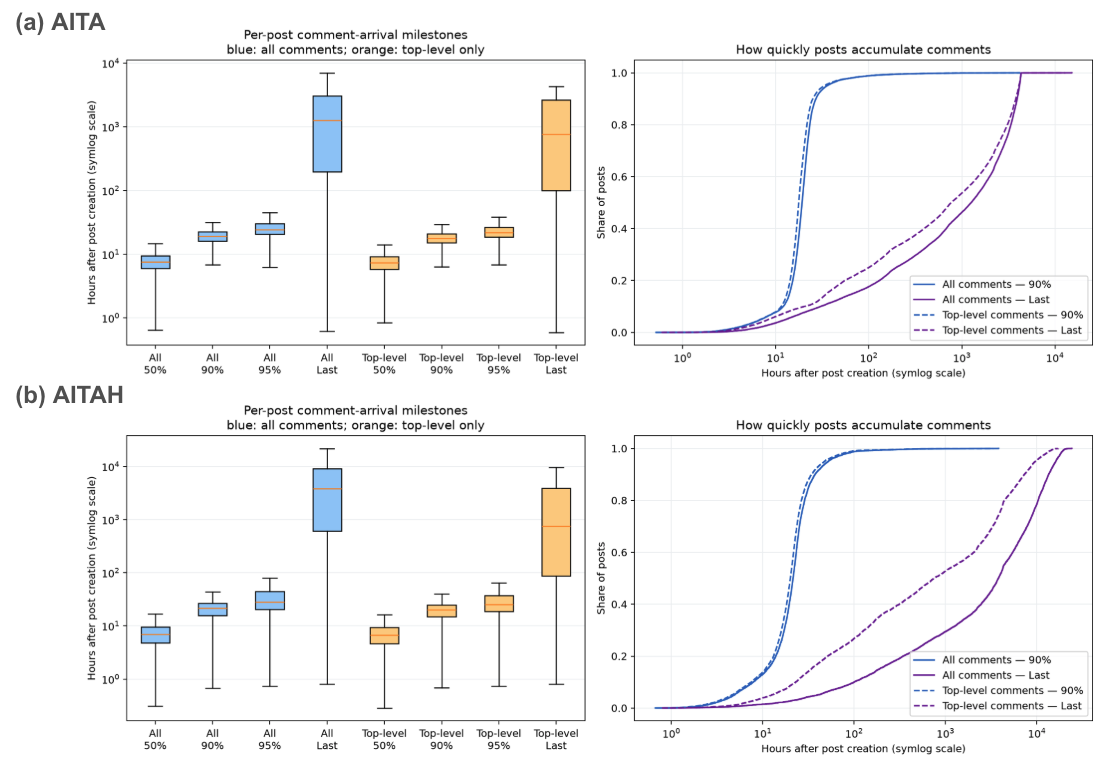
\includegraphics[width=\columnwidth]{figures/comment_timing.png}
  \caption{Comment timing in (a) AITA and (b) AITAH. Both communities collect
  most top-level comments within the first day, and AITA's $18$-hour verdict
  threshold falls near the point at which a typical post has received $90\%$ of
  them.}
  \label{fig:timing}
\end{figure}
